\documentclass[tikz,border=6pt]{standalone}
\usepackage[T1]{fontenc}
\usepackage{helvet}
\renewcommand{\familydefault}{\sfdefault}
\usepackage{tikz}
\usetikzlibrary{positioning}

\definecolor{ink}{HTML}{1F2937}
\definecolor{muted}{HTML}{6B7280}
\definecolor{head}{HTML}{1E3A5F}
\definecolor{prov}{HTML}{1D4ED8}
\definecolor{provbg}{HTML}{EFF6FF}
\definecolor{enc}{HTML}{047857}
\definecolor{encbg}{HTML}{ECFDF5}
\definecolor{outc}{HTML}{5B21B6}
\definecolor{outbg}{HTML}{F5F3FF}

\begin{document}
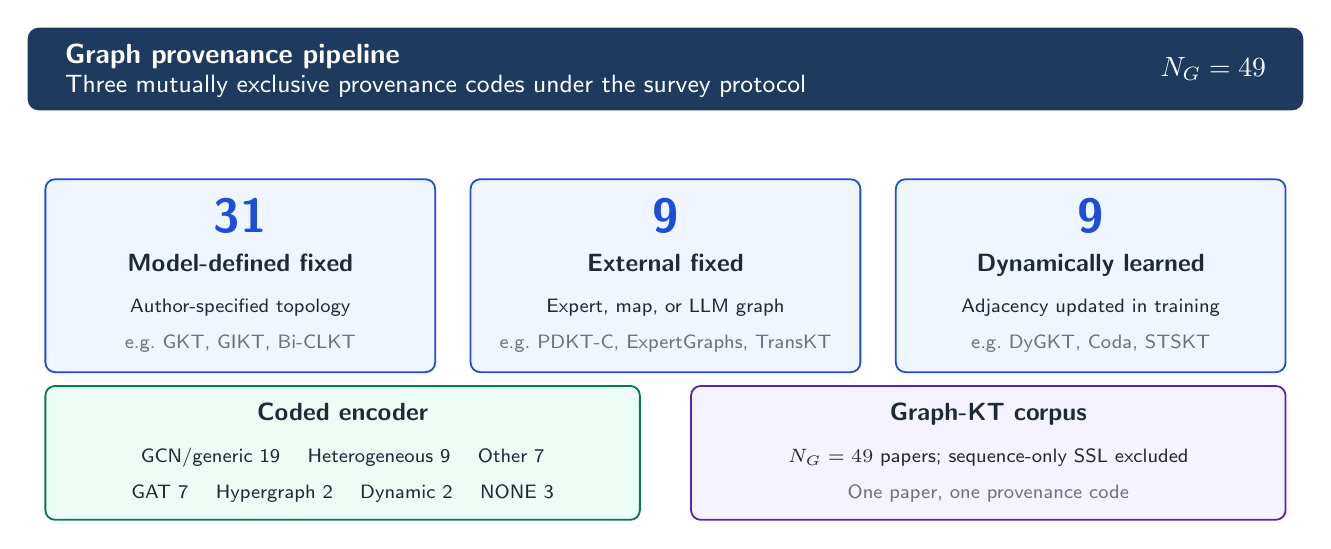
\begin{tikzpicture}[font=\sffamily]

\tikzset{
  pcard/.style={rectangle, rounded corners=3.5pt, align=center,
    minimum width=4.95cm, minimum height=2.45cm, inner sep=6pt,
    draw=prov, fill=provbg, line width=0.65pt, text=ink},
  ecard/.style={rectangle, rounded corners=3.5pt, align=center,
    minimum width=7.55cm, minimum height=1.70cm, inner sep=5pt,
    draw=enc, fill=encbg, line width=0.65pt, text=ink},
  ocard/.style={rectangle, rounded corners=3.5pt, align=center,
    minimum width=7.55cm, minimum height=1.70cm, inner sep=5pt,
    draw=outc, fill=outbg, line width=0.65pt, text=ink}
}

\fill[head, rounded corners=4pt] (0,0) rectangle (16.2,1.05);
\node[anchor=west, text=white, font=\sffamily\bfseries] at (0.35,0.68)
  {Graph~provenance~pipeline};
\node[anchor=west, text=white!88, font=\sffamily\small] at (0.35,0.30)
  {Three mutually exclusive provenance codes under the survey protocol};
\node[anchor=east, text=white, font=\sffamily\bfseries] at (15.85,0.52) {$N_G=49$};

\node[pcard] (c1) at (2.70,-2.10) {%
  {\color{prov}\fontsize{16}{18}\selectfont\bfseries 31}\\[2pt]
  {\small\bfseries Model-defined fixed}\\[3pt]
  {\scriptsize Author-specified topology}\\[1pt]
  {\scriptsize\color{muted}e.g.\ GKT, GIKT, Bi-CLKT}};
\node[pcard] (c2) at (8.10,-2.10) {%
  {\color{prov}\fontsize{16}{18}\selectfont\bfseries 9}\\[2pt]
  {\small\bfseries External fixed}\\[3pt]
  {\scriptsize Expert, map, or LLM graph}\\[1pt]
  {\scriptsize\color{muted}e.g.\ PDKT-C, ExpertGraphs, TransKT}};
\node[pcard] (c3) at (13.50,-2.10) {%
  {\color{prov}\fontsize{16}{18}\selectfont\bfseries 9}\\[2pt]
  {\small\bfseries Dynamically learned}\\[3pt]
  {\scriptsize Adjacency updated in training}\\[1pt]
  {\scriptsize\color{muted}e.g.\ DyGKT, Coda, STSKT}};

\node[ecard] (enc) at (4.00,-4.35) {%
  {\small\bfseries Coded encoder}\\[3pt]
  {\scriptsize GCN/generic 19 \quad Heterogeneous 9 \quad Other 7}\\[1pt]
  {\scriptsize GAT 7 \quad Hypergraph 2 \quad Dynamic 2 \quad NONE 3}};
\node[ocard] (out) at (12.20,-4.35) {%
  {\small\bfseries Graph-KT corpus}\\[3pt]
  {\scriptsize $N_G=49$ papers; sequence-only SSL excluded}\\[1pt]
  {\scriptsize\color{muted}One paper, one provenance code}};

\end{tikzpicture}
\end{document}
